\section{Squadratore e campionatore}
	Dopo aver effettuato le verifiche precedenti è stato montato il 
	circuito in 
	\figurename{ \ref{fig:sqd} }
	impiegando le componenti circuitali corrispondenti.
	
	\begin{figure}[ht]
		\centering
		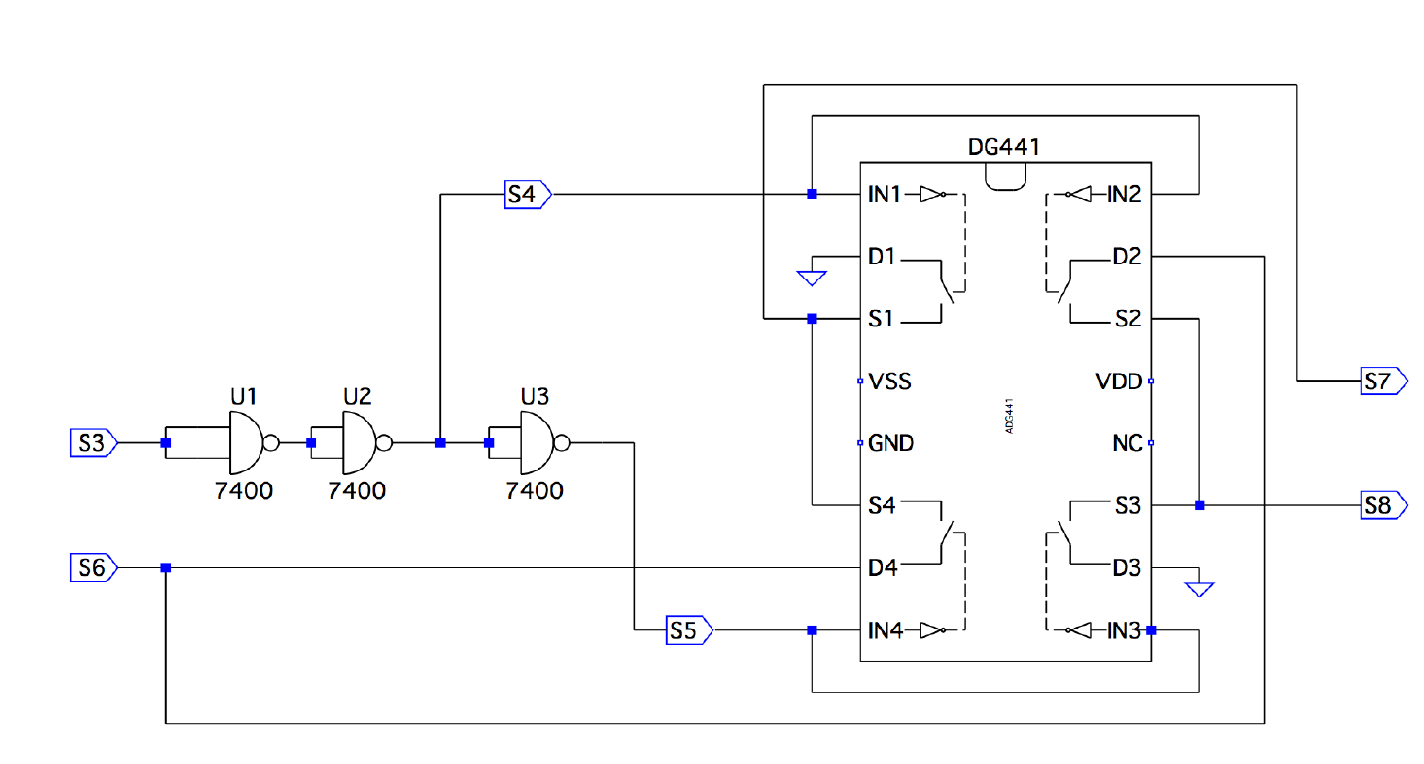
\includegraphics[scale=0.25]{deriv.png}
		\caption{Circuito che svolge la funzione di squadratore e campionatore}
		\label{fig:sqd}
	\end{figure}

	Il circuito costruito svolge la funzione di squadrare e campionatore la tensioni immesse.
	
	Si è proceduto pertanto alla verifica del funzionamento circuitale.
	Sono state d'apprima acquisite le forme d'onda visualizzabili su $S4-S5$
	ottenendo come da attese due segnali in opposizione di fase.
	\figurename{ \ref{f:s4-s5} }
	
	\begin{figure}[ht]
		\centering
		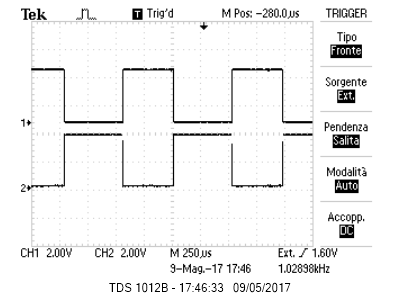
\includegraphics[scale=0.35]{s4-s5.png}
		\caption{segnale su s4 ch.1, s5 ch.2 }
		\label{f:s4-s5}
	\end{figure}
	
	Dopodiché sono stati acquisiti i segnali visualizzabili sui terminali $S7$ e $S8$
	per le due diverse posizioni del deviatore.
	
	Come è possibile vedere dalla \figurename{\ref{fig:s7}} si ottiene che i due segnali, qualora il
	deviatore sia collegato ad $S2$,  risultino dovuti alle semi-onda
	positiva o negativa, a seconda della traccia in esame.
	
	Per il deviatore collegato ad $S1$
	si attendono invece segnali a media nulla; le tracce ottenute risulta in buon accordo 
	con le attese.
	
	La presenza di spike in \figurename{\ref{fig:S7a}} e la non perfetta corrispondenza della media dei segnali a $0$ in \figurename{\ref{fig:S7b}} è stata imputata alla non idealità 
	degli operazionali impiegati nei montaggi circuitali.
	\begin{figure}[h]
		\centering
		\subfloat[ch.1 S7 ch.2 S8. Deviatore collegato a $S2$ ]{
			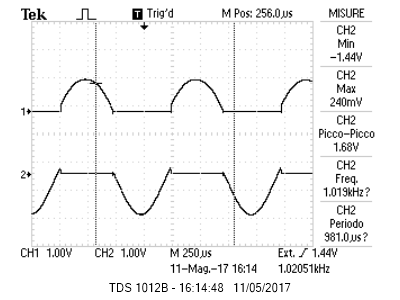
\includegraphics[scale=0.45]{s7-s8a.png}
			\label{fig:S7a}
		}
		\subfloat[ch.1 S7 ch.2 S8. Deviatore collegato ad $S1$]{
			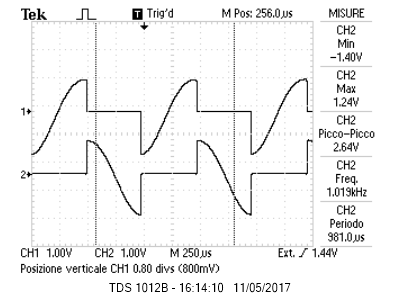
\includegraphics[scale=0.45]{s7-s8b.png}
			\label{fig:S7b}
		}
		\caption{Segnali acquisiti di $S7-S8$}
		\label{fig:s7}
	\end{figure}
